%! TEX root = main.tex

% this section has inline code block, we use this style
\lstset{language=C++, basicstyle=\ttfamily\bfseries\small\color{black}}

AmgXWrapper~\cite{chuang_amgxwrapper:_2017} bridges NVIDIA's AmgX library and PETSc, the linear algebra library used in PetIBM\@.
AmgX provides algebraic multigrid preconditioners and linear solvers for multi-GPU systems.
AmgXWrapper aims at providing painless integration of AmgX into legacy PETSc applications.
With AmgXWrapper, only four additional code lines are usually required in PETSc applications to use AmgX:\@ \lstinline{initialize}, \lstinline{setA}, \lstinline{solve}, and \lstinline{finalize}.

In addition to bridging AmgX and PETSc, AmgXWrapper also implements a matrix consolidation mechanism for the situation when there are more MPI processes (i.e., CPU cores) than GPUs.
This use case happens, for example, when a program constructs matrices and vectors in parallel with 32 CPU cores per compute node, but there are only 2 GPUs per node available to solve the matrix system.
Theoretically speaking, the linear solver lives on GPUs entirely, so the solving times should be the same regardless of how many CPU cores are involved.
However, when using AmgX directly in MPI-based code, the solving time increases when the number of CPU cores increases due to resource competition on a GPU\@.
Figure~\ref{fig:amgxwrapper-cons} shows the wall time of solving Poisson problems with fixed numbers of GPUs but with different CPU core numbers.

\begin{figure}[hbt!]%
    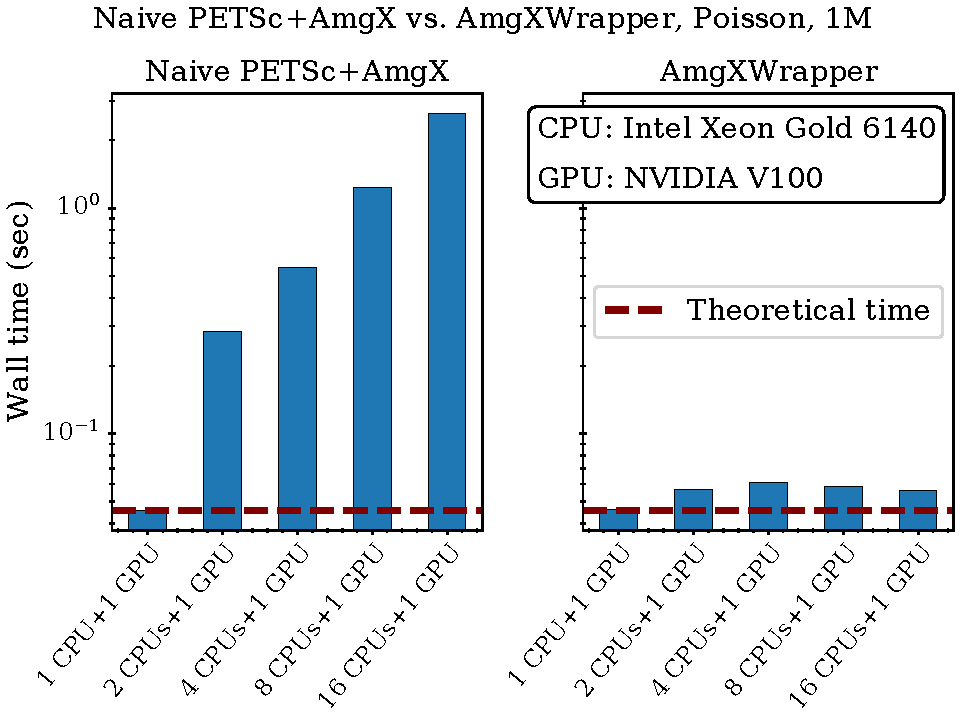
\includegraphics[width=\linewidth]{amgxwrapper-consolidation-tests-poisson-1M}%
    \caption{AmgXWrapper benchmark: 3D Poisson problem w/ 1M unknowns and using 1 V100 GPU.}\label{fig:amgxwrapper-cons-1M}%
\end{figure}
\begin{figure}[hbt!]%
    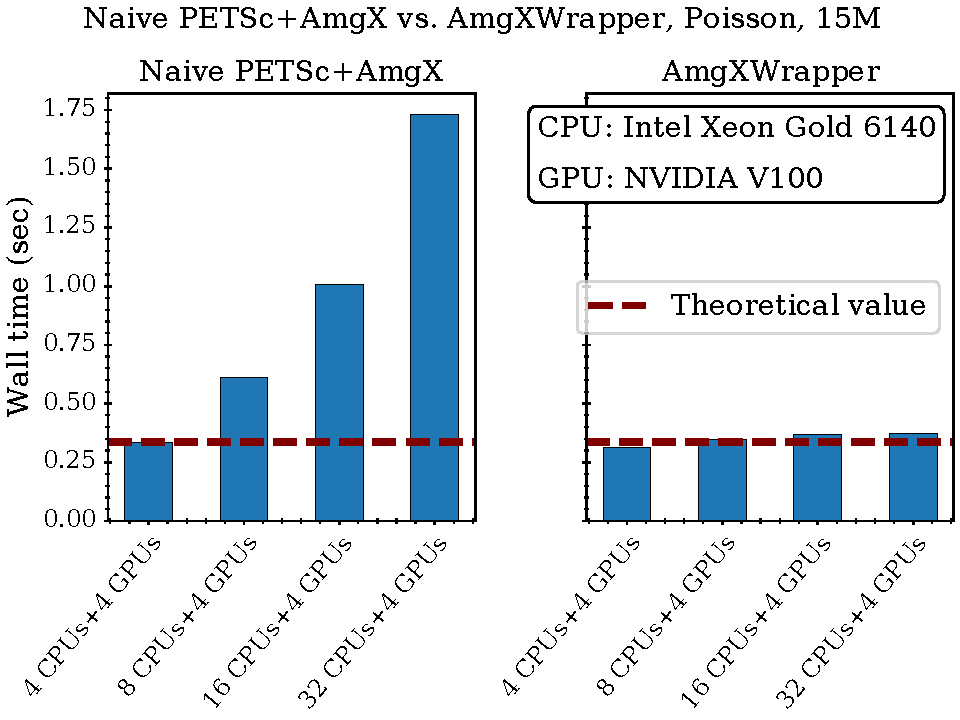
\includegraphics[width=\linewidth]{amgxwrapper-consolidation-tests-poisson-15M}%
    \caption{AmgXWrapper benchmark: 3D Poisson problem w/ 15M unknowns and using 4 V100 GPUs.}\label{fig:amgxwrapper-cons-15M}%
\end{figure}

The left figures of both figures~\ref{fig:amgxwrapper-cons-1M} and~\ref{fig:amgxwrapper-cons-15M} show that using AmgX naively, the wall times increase when the numbers of CPU cores increase. 
The figures on the two subplots' right show that with AmgXWrapper's consolidation mechanism, the wall times remain relatively constant regardless of the numbers of CPU cores.
Please refer to~\cite{chuang_amgxwrapper:_2017} for the explanation of AmgXWrapper's consolidation mechanism.

Figure~\ref{fig:amgxwrapper-speedups} shows the results of speedup/performance benchmarks.
Figure~\ref{fig:amgxwrapper-speedups-15M} shows the speedups of solving a small 3D Poisson problem that fits into one compute node, and figure~\ref{fig:amgxwrapper-speedups-33M} shows that of solving a bigger 3D problem with multiple compute nodes.
The compute nodes have 36 cores of Xeon Gold 6140 CPU cores per node and 4 V100 GPUs per node.
The linear solver used for the CPU results is the BoomerAMG from Hypre~\cite{henson_boomeramg_2002}, which implements the same algorithms used by AmgX but on CPU\@.
Assuming a perfect intra-node scaling of Hypre, one V100 GPU has a performance equivalent to 65 pure CPU cores for the small Poisson problem (figure~\ref{fig:amgxwrapper-speedups-15M}).
However, intra-node scaling is far from perfect, as shown in figure~\ref{fig:amgxwrapper-speedups-15M}.
Therefore, 1 V100 is much more potent than a fat node with 65 CPU cores.
As for the larger problem (figure~\ref{fig:amgxwrapper-speedups-33M}), one node with four GPUs is roughly equivalent to nine pure-CPU nodes.
This estimation assumes the pure-CPU cluster uses low-latency network hardware, such as InfiniBand.
These results imply that using AmgX and GPU computing saves both computational and monetary costs because one standalone workstation of 4 GPUs is cheaper than a 9-node cluster with InfiniBand.
The management cost of one workstation with 4 GPUs is also cheaper than that of a 9-node cluster.

\begin{figure}[hbt!]
    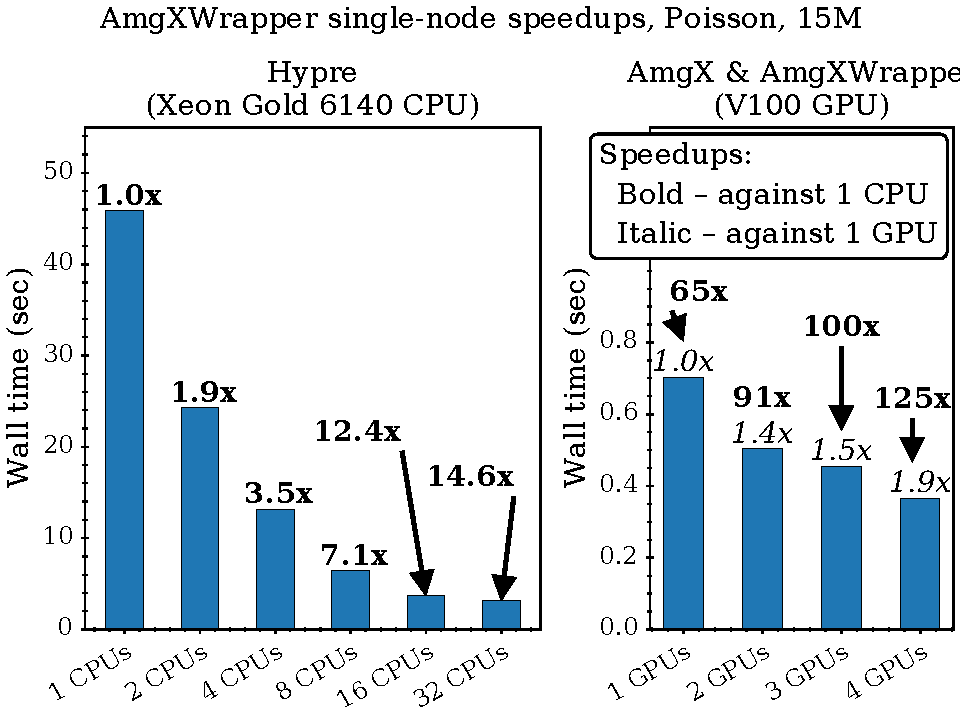
\includegraphics[width=\linewidth]{amgxwrapper-proc-speedups-poisson-15M}
    \caption{Speedups of AmgXWrapper vs.\@ Hypre w/ 15M unknowns.}\label{fig:amgxwrapper-speedups-15M}
\end{figure}

\begin{figure}[hbt!]
    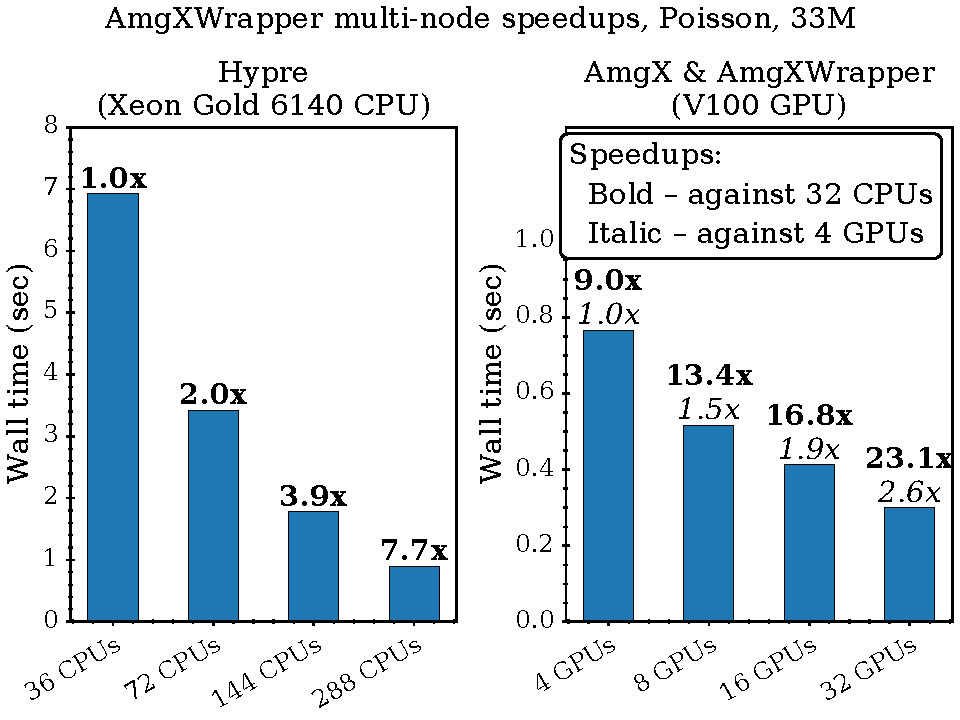
\includegraphics[width=\linewidth]{amgxwrapper-node-speedups-poisson-33M}
    \caption{Speedups of AmgXWrapper vs.\@ Hypre w/ 33M unknowns.}\label{fig:amgxwrapper-speedups-33M}
\end{figure}

% vim:ft=tex
